\chapter{Estrategia de la búsqueda}
\label{ch:estrategiaAuger}

En este capítulo se presenta la estrategia utilizada en la búsqueda de neutrinos ultra-energéticos con el Observatorio Pierre Auger.
Como fue presentado secciones previas, el m\'aximo desafío al detectar UHE$\nu$'s utilizando detectores de superficie es identificar los eventos que estos inician del inmensamente más poblado fondo de lluvias hadrónicas.
Esto puede lograrse separando las lluvias jóvenes, es decir, con presencia de componente electromagn\'etica, dentro de los eventos inclinados.

La figura \ref{fig:augerNu} resume los posibles canales de detección de neutrinos con el observatorio Pierre Auger, que ya fueron descriptos en la sección \ref{sc:easNu}.
	\begin{figure}[ht!]
		\centering
		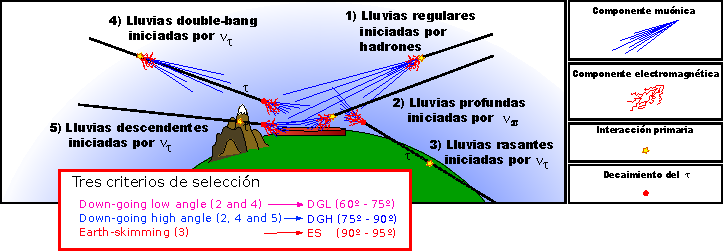
\includegraphics[width=\textwidth]{./fig/estrategiaAuger/auger_nu}
		% curveEarthSketch.png: 2404x1199 pixel, 150dpi, 40.70x20.30 cm, bb=0 0 1154 575
		\caption{\label{fig:augerNu}
		Esquema de los canales de detección de neutrinos con el SD del Observatorio Pierre Auger. Se detallan los tres análisis que fueron optimizados para identificar neutrinos provenientes de los diferentes rangos angulares.
		}
	\end{figure}
Debido a la diferencias esenciales que presentan estos canales de detección, en Auger existen actualmente tres búsquedas optimizadas para distintos rangos de ángulo cenital:
\begin{itemize}
 \item DGL: optimizado para buscar neutrinos down-going con ángulo entre $60^\circ$ y $75^\circ$.
 \item DGH: idem DGL pero para ángulos entre $75^\circ$ y $90^\circ$. 
 \item ES: optimizado para detectar neutrinos earth-skimming cuyo ángulo se encuentre entre $90^\circ$ y $95^\circ$.
\end{itemize}
%
Cada uno de estos an\'alisis ha dado lugar a una tesis doctoral. DGL fue encarado por Jos\'e Luis Navarro en el grupo de la Universidad de Granada~\cite{cite:tesisNavarro}. Mientras que DGH y ES han sido tomados por el grupo de la UBA, dando lugar a las tesis doctorales de Javier Tiffemberg~\cite{cite:tesisJavier} y Yann Guardincerri~\cite{cite:tesisYann}.

En los tres casos, la estrategia utilizada para la búsqueda fue del tipo \emph{análisis ciego}, cuyo procedimiento se esquematizan en la figura \ref{fig:strAuger}.
%
\begin{figure}[ht!]
	\centering
	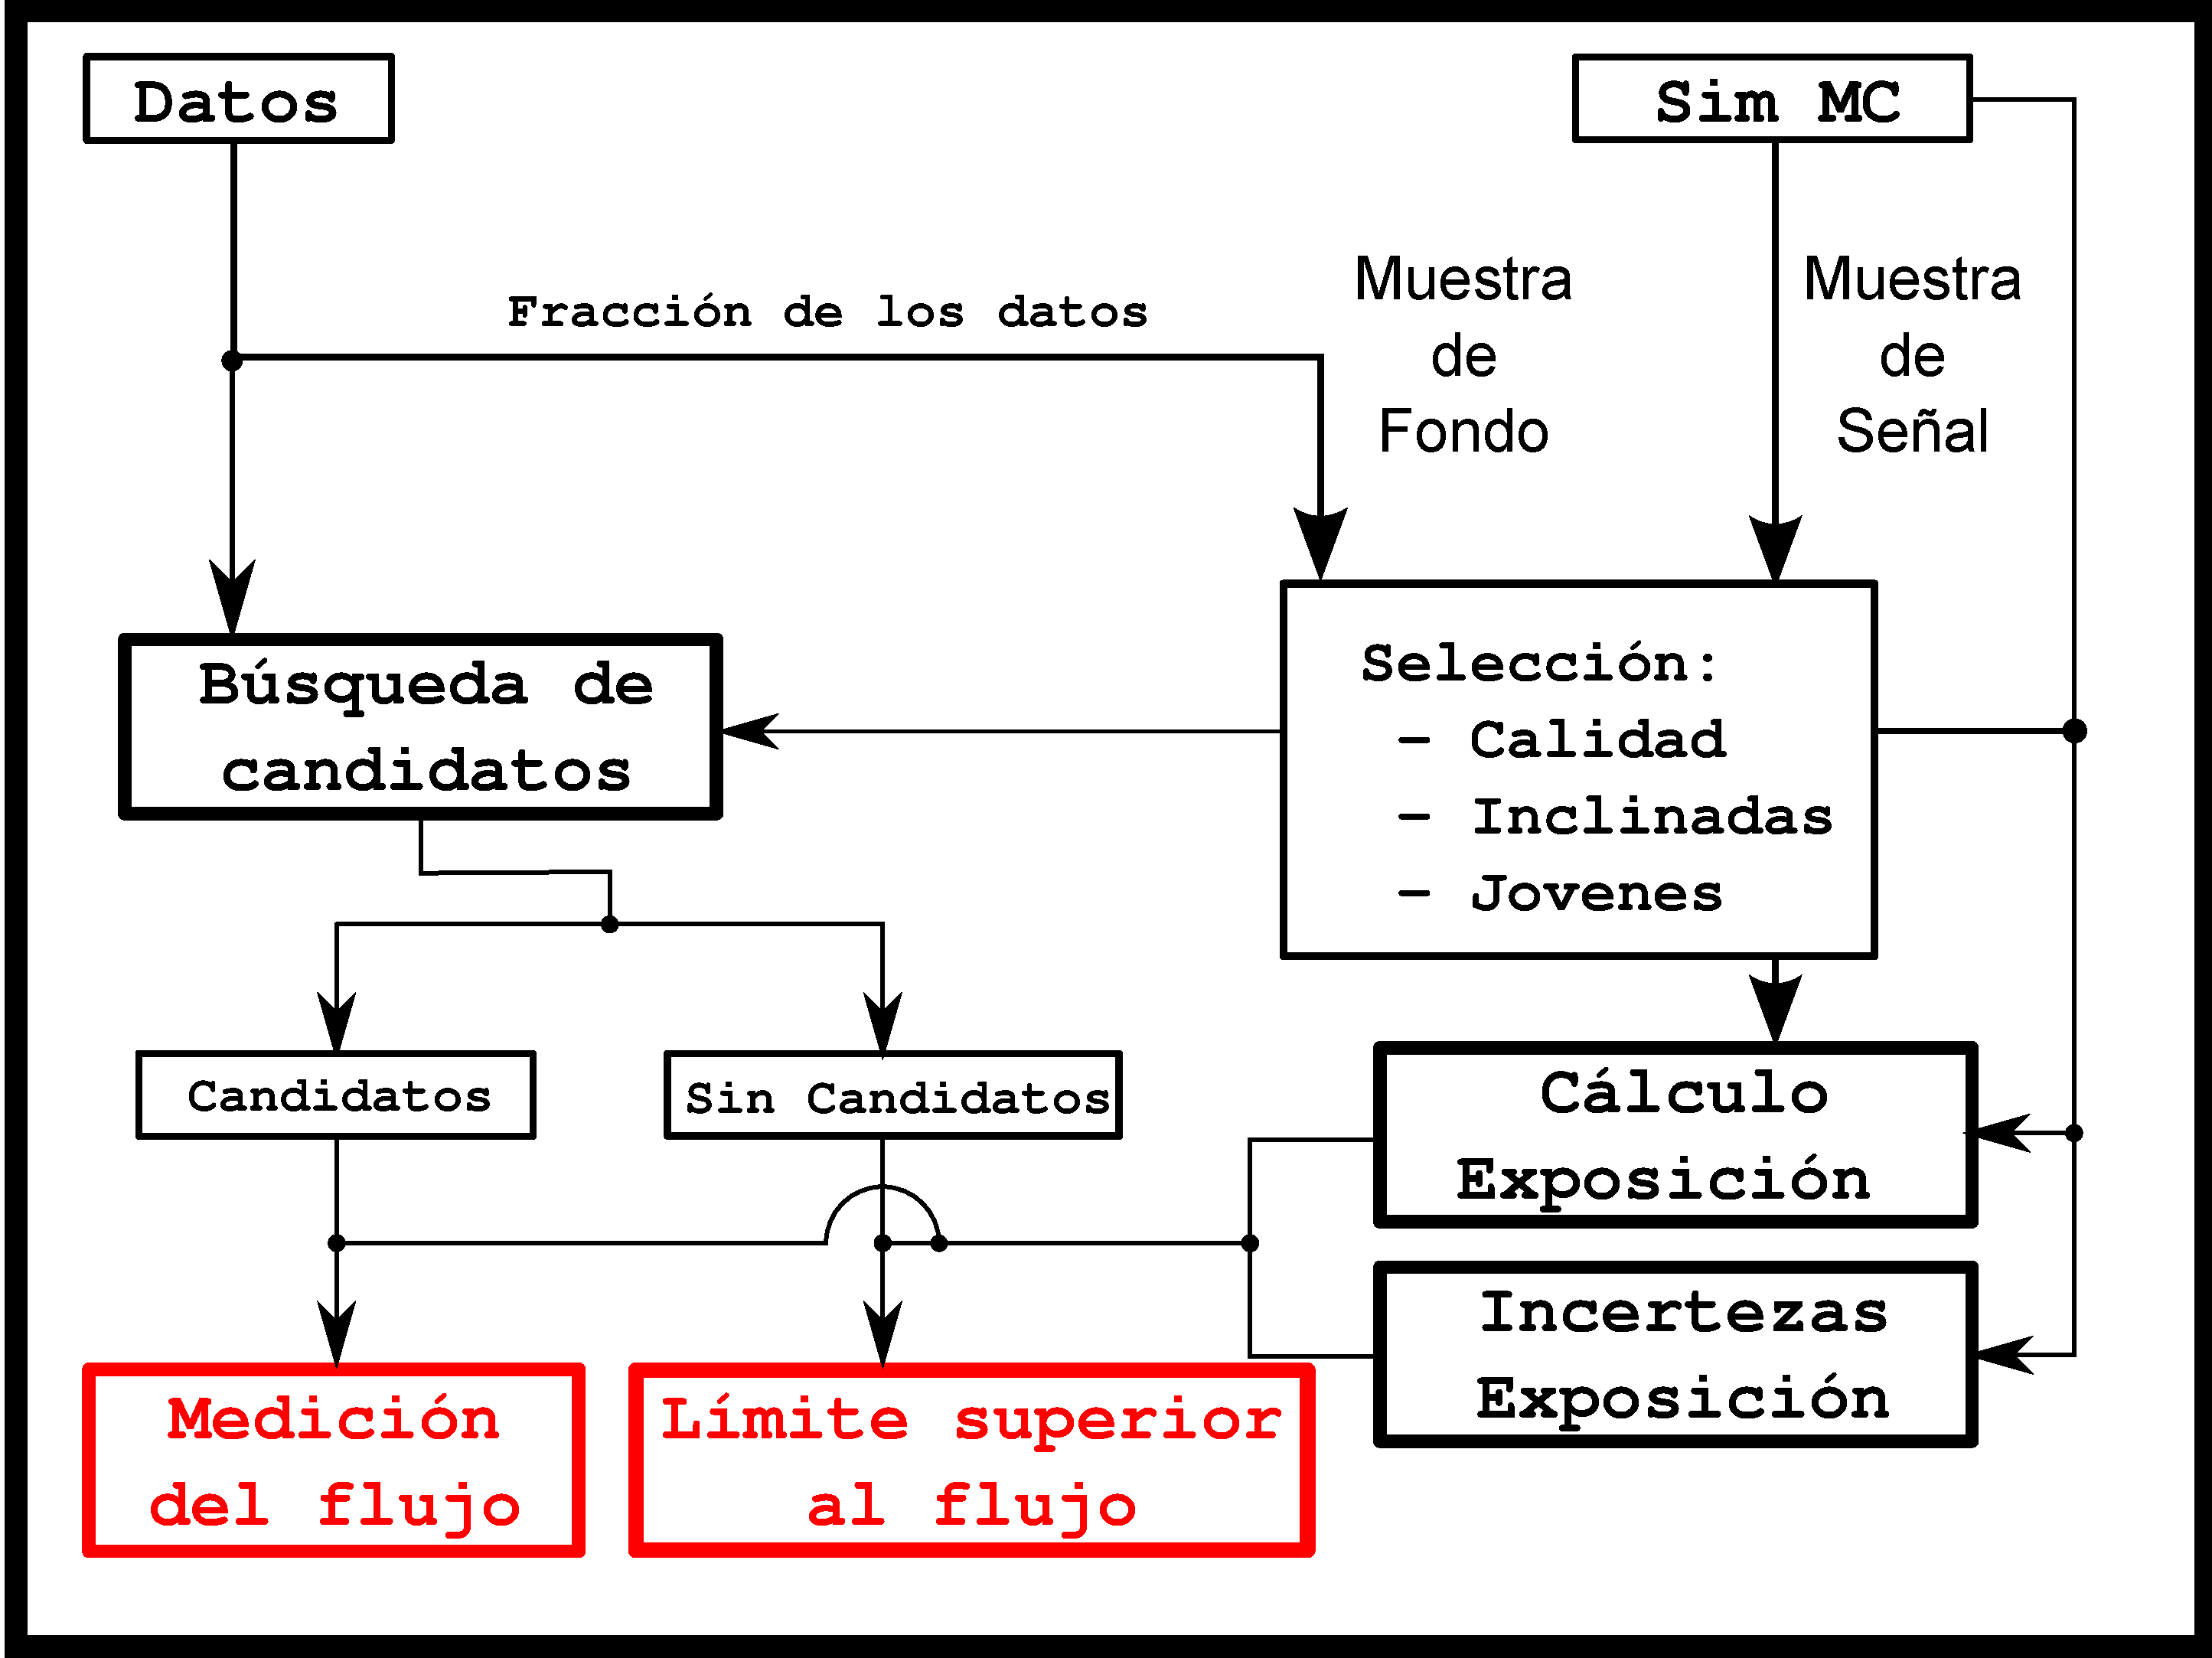
\includegraphics[width=\textwidth]{./fig/estrategiaAuger/analysisSchema}
	\caption{\label{fig:strAuger}
	Esquema de la estrategia utilizada en las búsquedas de neutrinos con el Observatorio Pierre Auger. Ver la explicación en el texto.
	}
\end{figure}
%
Aqu\'i la idea principal consiste en definir un criterio de selección, mediante el cual se decide si un evento es candidato a neutrino o no, sin utilizar datos o empleando una fracción peque\~na de los mismos que luego no podrá ser utilizada para realizar la búsqueda.
Luego es posible, por un lado, calcular con sus incertezas sistemáticas la exposición del detector a los distintos tipos de neutrinos, y por el otro, realizar la búsqueda de candidatos sobre los datos que no fueron utilizados en el entrenamiento del criterio.
Si hubiese candidatos en la muestra de b\'usqueda, sería posible informar la magnitud de el flujo con su error, o en caso contrario imponer un l\'imite superior a su valor.

Cabe destacar que para educar el criterio de selección es necesario contar con una muestra de señal (neutrinos) y otra de fondo (no neutrinos).
En los tres análisis se utilizaron simulaciones de Monte Carlo para generar la muestra de señal y una fracción de los datos como muestra de fondo.
% Este procedimiento, que emplea una parte de los datos para entrenar el m\'etodo, es lícito si los mismos son en su inmensa mayor\'ia no neutrinos y si el m\'etodo de entrenamiento no es sensible a outliers, condiciones que se satisfacen en los tres an\'alisis de Auger.
Luego, con las muestras de señal y fondo, se definieron criterios de calidad con el fin de eliminar eventos espureos y se optimizaron cortes en diferentes variables del detector que permiten elegir las lluvias jóvenes entre las inclinadas. 

En los próximos capítulos se abordarán las distintas etapas del análisis para las tres búsquedas.
Tambi\'en se presentar\'a su combinaci\'on y el c\'alculo de una \'unica exposici\'on a neutrinos ultra energ\'eticos con el Observatorio Pierre Auger.


% \textbf{XXX DEBERIA MENCIONAR LAS TRES TESIS EN ESTA SECCION ME PARECE. no estoy dejando claro en ningun lado en qué de todo lo que pongo trabaje.}
